\chapter{引言}\label{chap:introduction}

\section{问题的提出}\label{sec:intro_question}

近几十年来数据采集和存储技术突飞猛进,科学界可用数据总量和种类显著增加,挖掘数据中隐藏的信息非常具有挑战性,这是因为人类在给定时间内处理和分析大量数据的能力非常有限\citep{bougher2016machine}。很多自然现象是由多种因素所致,基于这些因素所构建的模型复杂度较高\citep{reitsma2010geoscience},因此人类很容易丢失一些从数据中捕获有效信息的机会,进而对复杂现象内在机制的理解存在一定的局限\citep{feyyad1996data}。

人类一直致力于理解自然现象的本质,期望在不同的条件下做出最优决策。过去几十年里,人类创造和收集的数据远超出了从数据中提取的信息量,很多模型的预测能力难以与数据增长的速度同步,因此数据的价值并未完全被开发出来。为了最大化利用爆炸式增长的数据,人类需要解决几个重要问题:(1)能够从大量数据中提取信息;(2)从数据中推导出的模型比传统的经验模型能获取到更多的信息;(3)这些信息需要遵循自然界普适性的规律。

人工智能(Artificial Intelligence,简称AI)是一个大领域,与任何智力工作相关。图灵测试指出,询问者在提出一些书面问题后,如果人类不能区分书面回答来自人类还是计算机,那么这台计算机就通过了测试\citep{turing2009computing}。图\ref{fig:intro_AI_ML}展示了AI、机器学习(Machine Learning,简称ML)和深度学习的逻辑关系。ML是AI的主流算法,深度学习又是ML近些年来发展最迅速的分支之一。本论文选择ML作为重点关注的技术,它是机器从数据中通过算法学习规律进而预测新数据的方法。

\begin{figure}[!htbp]
  \centering
  \noindent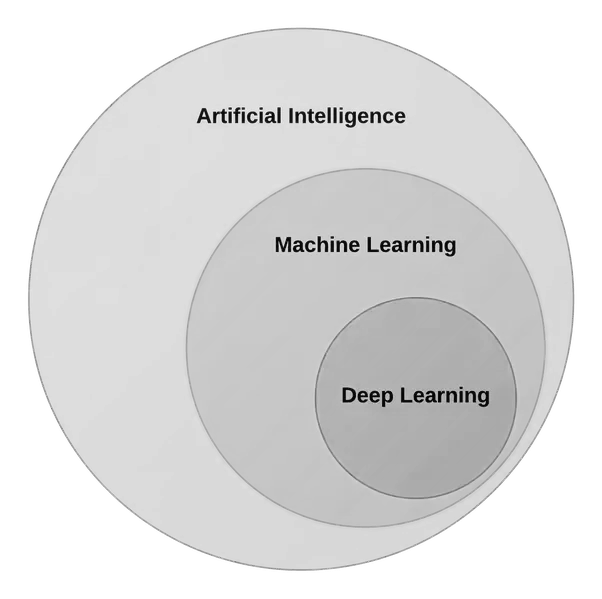
\includegraphics[width=0.45\textwidth]{Img/chap1_intro/AI_ML.png}
  \vspace{-0.6cm}
  \bicaption[人工智能、机器学习和深度学习的逻辑关系]{人工智能、机器学习和深度学习的逻辑关系。}{The relationship between artificial intelligence, machine learning and deep learning.}
  \label{fig:intro_AI_ML}
\end{figure}

根据目标任务的差异,ML可用于分类、回归、聚类和降维等问题;根据数据结构的差异,ML可以分为空间结构数据学习、序列结构数据学习和时空结构数据学习;根据数据是否带有标签以及标签的数量,ML又可分为监督学习、半监督学习和无监督学习等。监督学习处理的数据全部带有标记,常被用来处理分类和回归问题。ML中多数算法都属于监督学习,如线性回归(Linear Regression,简称LR)、支持向量回归(Support Vector Regression,简称SVR)、决策树(Decision Tree,简称DT)、随机森林(Random Forest,简称RF)、梯度提升回归树(Gradient Boosting Regression Tree,简称GBRT)、极端随机森林回归(Extra Trees Regression,简称ETR)、$k$近邻($k$-Nearest Neighbor,简称KNN)、卷积神经网络(Convolutional Neural Network,简称CNN)、长短期记忆神经网络(Long Short-Term Memory Recurrent Neural Network,简称LSTM-RNN)等。

很多自然现象可看作是一个复杂系统,例如气候变暖、地震发生机制等\citep{fan2021statistical}。现有的可操作且简化的经验模型通过降低复杂度(研究个别现象)或加强假设/近似进行推论,但对于大尺度系统的运行机制难以精准描述。ML模型排除了传统经验模型中人为干扰的因素,直接从数据中学习,进而为探究复杂现象提供了一条新的研究路径。

目前,机器学习在复杂问题中的应用领域较为广泛,这里重点关注地球科学领域。地球科学中很多数据集属于时空结构数据,例如大气模拟、海洋运输、火势蔓延、土壤运动、植被碳循环过程等,这些都是时空动力学领域内重要的研究问题\citep{mathieu2015deep,oh2015action};卫星图像的地形和纹理特征属于空间结构数据,类似于计算机视觉,研究对象通常具有一些描述边缘、纹理、形状和颜色等特征,利用这些特征构建机器学习算法,从而实现对象的定位、分类和检测等目标\citep{lee1990neural};地震波动态时间序列类似于自然语言与信号识别,属于时间序列数据\citep{rouet2017machine,perol2018convolutional,devries2018deep}。

根据数据出现的时间顺序排列的数据称为时间序列。时间序列预测基于时间结构数据,可利用机器学习分析时间序列数据。自然界中很多预测问题都涉及到时间因素。可通过时间序列推断过去数据点序列发生的事件,预测未来将会发生的事件。本论文根据数据复杂度的不同选取了几种时间序列数据,研究太阳黑子活动、龙子祠泉流量的动态趋势以及南加州地区中期地震预报。

\section{研究现状、挑战与机遇}\label{sec:intro_veiw}

深度学习兴起前,关于计算机视觉和语音识别等目标任务多数是基于人工设计的特征和典型的机器学习方法。在计算机视觉领域,常用的人工设计的特征包括SIFT、SURF、HOG、HOF、MBH等。人工设计的特性增强了对解释性驱动因素的控制,但这个过程繁琐,迁移能力差,结果可能是非最优的。与使用人工设计特征的算法相比,使用由数据驱动的机器学习有时非常有效。通常,机器学习算法在处理复杂任务方面优于物理模型,尤其是在物理机制不完善而观测数据较多时。机器学习可预测某时间段内相对静止的特征,也可用来研究动态变化过程。与半经验性的物理建模方法相比,机器学习少了人工的干预,使用起来更加灵活。

尽管机器学习常见的应用领域(计算机视觉和语音识别)与地球科学中的实际问题存在很多的相似之处,但还是有不同的方面。例如,计算机视觉处理的照片有三个通道(红绿蓝),但高光谱卫星图像会扩展到数百个光谱通道,远超出可见光范围,这与自然图像的统计特性不同;而且高光谱卫星图像的光谱通道存在空间上的依赖性,违反了数据独立同分布的重要假设;另外,由于地球科学研究中使用不同种类的传感器采集不同类型的数据,这些数据存在不同的成像几何、时空分辨率等特征,很难集成这些数据,而且多种类型的传感器收集到的观测数据存在噪声来源不同、数据丢失和系统偏差等问题。

一般地,机器学习需要具备以下几个要素:
\begin{enumerate}
  \item[$\circ$] \textbf{解释能力}。在解决实际问题时,不仅要考虑提高预测的精度,更要重点关注预测结果的可解释性。目前来说,可解释性是机器学习普遍存在的缺陷\citep{montavon2018methods}。机器学习从观测数据中得到的是统计相关关系,而不是因果关系\citep{runge2015identifying,reichstein2019deep}。为了提高机器学习的可解释性,我们需要挑选合适的输入特征;再者,基于神经网络的算法能够给出每个隐藏层的特征值,可视化这些特征值在一定程度上也能观测到算法学到的规则。
  \item[$\circ$] \textbf{泛化能力}。机器学习通常在训练时性能表现良好,但在外推时结果可能会出现很大的偏差,这可能是由过拟合或观测数据中存在的偏差所致\citep{friedlingstein2014uncertainties}。为达到预期的任务目标,可减小算法的规模或提供更丰富的数据。
  \item[$\circ$] \textbf{表达能力}。表达能力本质上是函数逼近。万能逼近定理指出,一层的神经网络几乎可以近似所有的连续函数。但一层的神经网络在实际应用时很难拟合。可通过增加网络层数和节点数获取更强表达能力的神经网络。
\end{enumerate}

一般地,物理建模和机器学习被看作是两类学科。前者由理论驱动建模,后者由数据驱动建模。在原理方面,物理方法可以解释;在适应数据方面,机器学习具备高度的灵活性。从机器学习发展趋势来看,物理建模和机器学习协同作用能够增加模型的可信度\citep{karpatne2017theory,karpatne2017physics,camps2018physics}。

\section{论文结构安排}\label{sec:intro_strcture}

本论文基于不同的时间序列数据,利用机器学习方法进行处理和分析,发现和理解新知识,推动机器学习在时间序列问题中的应用。第\ref{chap:ml_theory}章为机器学习理论部分,简要介绍论文涉及到的机器学习的技术原理和方法,然后引出这些算法训练前必要的准备条件。按照数据集的复杂程度,此后几个章节分别研究太阳黑子活动、泉流量变化趋势和地震中期数值预报。

第\ref{chap:ml_sunspot}章基于一种输入特征,利用神经网络探测太阳黑子活动。太阳黑子是太阳局部强磁场活动在太阳光球层上产生的黑色斑块,是太阳活动强弱的重要指标。太阳黑子活跃时会影响地球环境和人类经济发展。若人类能够提前预知太阳黑子活动并做出相应的防御措施,可以减少太阳活动带来的损失。从长期记录来看,近几十年来太阳黑子峰值呈现持续下降的趋势。为了继续跟踪太阳黑子活动,我们采用神经网络预测未来1个月、72个月太阳黑子活动。本论文中将未来72个月太阳黑子活动最剧烈时视为第25太阳周的峰值。这里重点关注第25太阳周太阳黑子活动的峰值。

第\ref{chap:ml_spring}章基于两种输入特征,利用机器学习预测龙子祠泉流量变化。近些年来,人类过度开采地下水,使部分泉水面临干涸的风险,因此合理管理地下水的用量就显得尤为重要。如果能够准确预知未来1个月甚至几个月地下水动态变化趋势,就能够最大化地管理地下水,从而实现地下水的可持续供应。龙子祠泉具备喀斯特地貌特征,地下水流路径错综复杂,基于半经验性的物理模型难以准确预测地下水变化趋势。机器学习擅长处理复杂问题,为预测龙子祠泉的地下水位提供了研究方法。

第\ref{chap:ml_seismic}章基于多种输入特征,利用机器学习对南加州地区进行地震中期数值预报。原始数据集为1932年至今的南加州地区地震目录。这里选择了中期预报,是因为长期预报需要长时间的数据资料积累(南加州地区地震目录记录最长年限为$\sim$90年),而短期预报机制更加复杂。基于地震目录我们得到16个地震因子,其中7个地震因子与空间地震分布密切相关。基于这些地震因子,我们尝试探索未来可能发生的最大震级。

第\ref{chap:conclusion}章分别对太阳黑子活动、泉流量动态变化和地震中期数值预报这几个目标任务进行了总结与展望。需要指出的是,本论文中很多关于统计学、机器学习中的专业术语并未加以详细区分,比如算法/模型/方法/映射、机器学习/神经网络/深度学习、训练/优化/拟合/模拟/学习等。论文中这些含义近似的术语将会被无差别使用。
